\section{Semantics Aware Representation Learning}
이번 섹션에서는 vector representation E 를 학습시키기 위한 방법들을 설명한다. E를 우리의 의도대로 임베딩시키기 위해 제안되었던 방법들과 각 방법 별 문제점, 그리고 해결하기 위한 방법들을 나열하였다. 그리고 우리가 설계한 최종 목적함수와 constraint 를 소개한다. 

\subsection{Semantic Spaces for Malwares}

\textbf{Definition. }
Let $X = \{x1, …, x_n, …, x_N\}$ be a set of malwares.
Let $E$ and $S$ be a subset of vector space of dimension d and let semantic component set $S = \{s_1, ... , s_k, … s_K\}$ be a basis for $E$. We have constraints for $s_i$ whose l2 norm is one, $||s_i||_2 = 1$ and all semantic components are linearly independent.  
Then for every $e \in E$, there is an unique linear combination of the sementic component vectors that equals $e$.
\[
e = c_1*s_1 + c_2*s_2 + … + c_k*s_k 
\]

where $c_i$ is the i’th element of coefficient vector $ C = \{c_1, …, c_i, …, c_k\}$
We call a vector $e$ as a semantics of malware $x$ and there is a nonlinear mapping from $X$ to $E$. 

\textbf{Metric function}
we use an Euclidean Distance $d(e_i, e_j)$ for a metric of a set E and it means the function that defines a distance between  semantics of two malwares. 



\subsection{Solution Overview}
피규어다.
% Figure
\begin{figure*}
  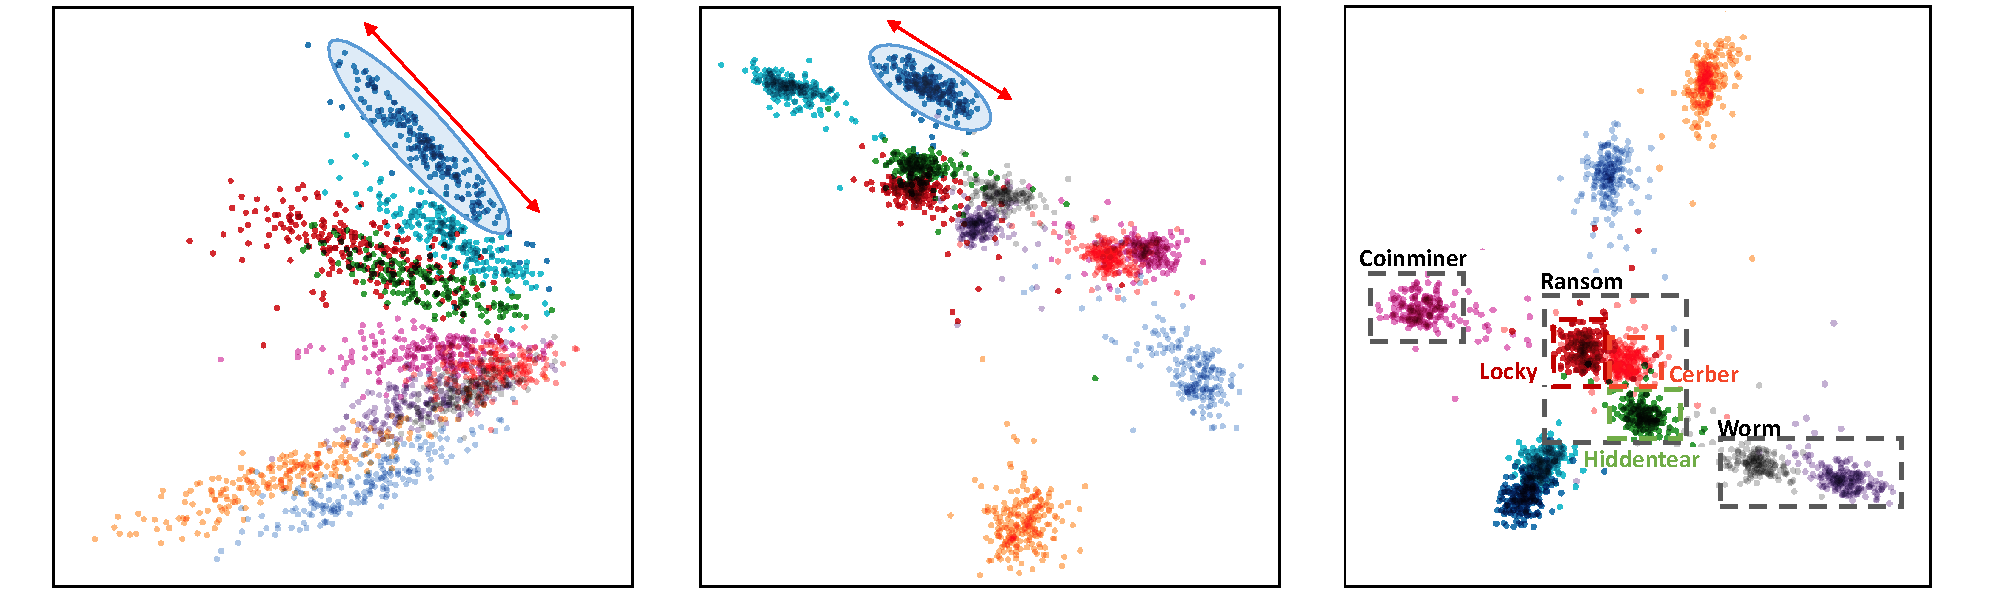
\includegraphics[width=\textwidth]{../figures/concept.pdf}
  \caption{concept}
  \label{fig:three}
\end{figure*}


\textbf{Multilabel Classification. }
멀웨어 샘플의 의미를 반영하는 Vector representation E 를 학습시키기 위해 멀티레이블 분류 학습을 Auxiliary Task 로 선택하였다. 이 분류 태스크를 학습하기 위해 뉴럴 임베더 h는 표현 벡터들을 선형 분류기가 분류할 수 있도록 위치시킨다. 기존 대부분의 멀웨어 분류기를 학습하는 연구들은 하나의 레이블로 분류하도록 분류기를 학습한다. 하지만 멀웨어 도메인에서 하나의 레이블을 특정하고 이를 기준으로 가르치는 Auxiliary Task로 Malware IR System 을 만든다면, 학습하는 임베딩 벡터가 그 샘플의 의미를 담기에 부족한 점이 있다. 첫 째, 멀웨어에 레이블링을 하는 프로세스가 멀웨어의 의미를 표현하는데에 합리적이지 못하다. 멀웨어를 대분류, 중분류, 소분류 등 하이러키컬한 분류 체계를 갖도록 레이블링 하는 경우가 대부분이다. 하지만 실제로 멀웨어는 여러 의미를 갖고 있고, 

첫 째는 하나의 레이블이 만약 Trojan이나 Adware 같은 대분류라면 같은 분류 안의 샘플들을 좀 더 세세하게 구분하여 information retrieval task 를 수행할 때에 정확하게 같은 의미의 샘플을 검색하기가 쉽지 않다. 샘플들의 벡터의 차이가 정확하게 어떤 의미인지를 알 수 없기 때문이다. 레이블이 만약 소분류라면 거의 동일한 샘플들만 같은 분류 안에 속해있을 가능성이 높고, 분류의 개수가 너무 많기 딥러닝 모델의 캐퍼시티가 충분하다면 샘플들을 외우고 하이러키컬 representation 을 학습하지 않아 Generalization 효과가 떨어지게 될 것이다. 따라서 의미적으로 정확하게 같은 샘플들은 검색될 수 있지만 의미가 비슷한, 동일하지 않은 샘플들에 대해서는 검색되지 않는다. 따라서 우리는 같은의미를 가진 샘플들 뿐만 아니라 비슷한 의미를 가진 멀웨어 샘플들에 대해서도 검색이 가능하도록 하기 위해 멀티 레이블을 분류하도록 Auxiliary Task 를 학습시켜 얻은 Vector representation 을 사용한다. 이는 여러 의미 계층에 대한 공통 피쳐를 딥러닝 모델이 모두 학습할 수 있게 되기 때문에 가능해진다. 

% 하나의 레이블을 붙이는 과정 자체가 비합리적이다. 일관되지 않다. 네이밍을 하는 순간 다른 정보가 다날라간다.  


\textbf{Centerloss. }
Auxiliary task 로 임베딩한 샘플들이 inner class variance 가 너무 커서 ranking module 에서 같은 클래스 내 두 샘플의 거리가 서로 다른 클래스 내의 두 샘플 간 거리보다 더 커지는 현상이 발생하게 된다. 이 문제를 해결하기 위해 우리는 메트릭 러닝을 위한 목적함수를 추가하여 최종 목적함수를 세팅하였다. 센터로스[ref]를 변형한 목적함수를 통해 innerclass variance 를 낮추고 상대적으로 인터클래스의 거리는 멀어진다. 

싱글레이블 센터로스를 제안했던 논문에서는 각 레이블 별로 템플릿 벡터를 익스터널 메모리에 저장해놓고 그 템플릿 벡터와 보틀넥의 거리가 작아지도록 MSE 에러를 로스에 추가했다. 우리도 마찬가지로 각 레이블별로 시멘틱 컴포넌트 벡터를 익스터널 메모리에 저장해놓고, 보틀넥이 정답 레이블 벡터들의 합이 되도록 MSE 에러를 로스에 추가했다. 그리고, 보틀넥과 정답 레이블벡터의 합의 차이에 alpha/the number of answer labels 만큼의 곱을 하여 각 레이블을 업데이트해준다. 알파는 하이퍼파라미터로, 템플릿 벡터와 보틀넥을 얼마나 섞어서 기존 템플릿벡터를 업데이트할지를 결정해주는 값이다. 

\textbf{Consider the importances of labels. }
agent 나 downloader같은 태그들에 대한 innerclass variance 를 낮추는 것보다는 오히려 수는 적지만 중요한 태그들인 ransom, coinminer 등의 태그들의 innerclass variance 를 줄이는 것이 Ranking 할 때 더 의미가 있다. 따라서 태그들의 중요도를 constraint 로 추가한 Centerloss 를 사용한다. 
원래 리트리벌에서 랭킹을 위한 스코어링은 원래 하는짓인데 이걸 딥러닝에서 되게 한건 노블한거다. 연역적으로 왜 이렇게애해야하는지는 자명하다.


\textbf{뭘 검색할 수 있어야 우리가 앞에서 문제라고 했던 애들이 해결된다. 연산한걸 검색할 수 있고,...} 




\subsection{Proposed Objective Functions : Multilabel Center Loss}
Overview 에서 설명했던 방법들을 합쳐서 

\textbf{Multilabel Center Loss}

\textbf{Multilabel Weighted Center Loss}

\begin{equation}
\label{eqn:06}
\min_{\theta, w, b} J(\theta, w, b) = -\sum_i{ \sum_j{ y_{mij} \log{\hat{y_{ij}}}}}
\end{equation}

s.t.

\[
h(v_i;\theta)) - \sum_k{c_{ik}} < \epsilon ,
\]


\[
||c_i||_2 = cc_i
\]

for

\[
 i = \{1,2,3, ..., N\}
\]

위의 constrained optimization problem 의 Lagrangian 은 다음과 같다.

\begin{equation}
\label{eqn:07}
\begin{split}
L(\theta, w, b, \lambda_1, \lambda_2) = -\sum_i{[ \sum_j{ y_{mij} \log{\hat{y_{ij}}}}} \\  
+ \lambda_1 * (\sum_k{c_{ik}} - h(v_i;\theta))^2 + \lambda_2 * (||c_i||_2 - cc_i)^2 ]
\end{split}
\end{equation}

where 
\[
\hat{y_{ij}} = \frac{exp(w*h(v_i;\theta)+b)}{ 1 + exp(w*h(v_i;\theta)+b)}
\]

실제로 학습할때 메모리에 새로운 레이블 템플릿 벡터를 다음의 방법으로 업데이트하여 두 번째 constraint를 강제로 만족시켰다. 
\begin{equation}
\label{eqn:08}
c_i \leftarrow c_i + (1-\alpha) * (e_i - \sum_k{c_{ik}}) \\  
\end{equation}


\textbf{The meaning of averaging center vectors. }

\textbf{The meaning of adding center vectors. }


